\documentclass[12pt,a4paper]{article}
\usepackage{tpl}
\usepackage{chessboard}
\dbegin{Кружок для 7 класса, начинающие, школа №179}{Решения занятия №16}

\z Какое наименьшее количество детей может заниматься в кружке, если известно, что девочек в нём больше $40\%$, но меньше $50\%$?

\s Если в кружке 3 девочки и 4 мальчика, то девочек приблизительно $42\%$. Для чисел $n<7$ можно перебрать все дроби со знаменателем $n$ и получить, что они не лежат в интервале $(\frac{2}{5};\frac{1}{2})$.\QEDA\\

\z Какое наибольшее количество клеток в квадрате $8\times8$ можно закрасить так, чтобы в каждом уголке из трёх клеток была по крайней мере одна незакрашенная клетка?

\s Разобьём квадрат на 16 квадратов $2\times2$. В каждом из них не больше 2 закрашенных клеток, значит, всего закрашено не более 32 клеток. Пример на 32 клетки --- те клетки, которые белые на шахматной доске.\QEDA\\

\n В город приехали 60 певцов из двух стран --- Франции и Германии. Каждый день два певца из разных стран дают концерт, при этом пары певцов не должны повторяться. Какое наибольшее количество концертов они смогут дать?

\s Можно считать, что певцов из Германии не больше. Пусть их $30-k$, тогда певцов из Франции $30+k$. Тогда максимальное количество концертов --- $(30-k)(30+k)=900-k^2$. Это число максимально, когда $k=0$ и равно 900.\QEDA

\p То же, но певцов 75.

\s Аналогично предыдущему пункту получаем, что если певцов из Германии $37.5-k$, то концертов $37.5^2-k^2$. При этом $k$ должно быть полуцелым и при этом не целым, то есть $k^2\geq\frac14$. Значит, максимум этого выражения равен $37\cdot38=1406$.\QEDA\\

\z Город представляет из себя квадрат $3\times3$, в котором каждая сторона квартала --- участок улицы длины 500 метров. Какой наименьший путь придется проделать катку, чтобы заасфальтировать улицы?\label{katok}

\s Чтобы каток мог пройти весь город, должно быть не более 2 перекрёстков, из каждого из которых выходит нечётное количество дорог. У нас таких перекрёстков 8, значит, нужно соединить их ещё как минимум 3 дорогами, а минимальная длина дороги --- 500 метров. Значит, меньше чем $13.5$ километрами обойтись не получится. Пример на $13.5$ километров изображён ниже.\QEDA\\

\z На доске написаны числа от 1 до 100. Петя хочет выбрать из них несколько чисел так, чтобы разность двух любых выбранных чисел была составным числом. Какое наибольшее количество чисел он сможет выбрать?

\s Заметим, что мы не можем выбрать 2 числа с разностью меньше 4. Поэтому если мы выбрали какой-то набор чисел $a_1<a_2<\ldots<a_k$, то $99\geq a_k-a_1\geq 4(k-1)$, откуда $k\leq 25$. Пример на 25 --- все числа, кратные 4.\QEDA\\

\z Новогодняя гирлянда состоит из красных и синих лампочек. Рядом с каждой красной лампочкой есть хотя бы одна синяя. Какое наибольшее количество красных лампочек может быть в гирлянде, если всего лампочек 60?

\s Пусть красных лампочек $k$. Рассмотрим $k$ пар <<красная лампочка --- соседняя с ней синяя лампочка>>. Каждая синяя лампочка участвует не более чем в двух парах, значит, всего лампочек минимум $\frac{3k}{2}$, т.е. $k\leq40$. Пример на 40 --- 20 троек, в каждой из которых сначала красная лампочка, потом синяя, потом красная.\QEDA\\

\newpage
\z Какое максимальное количество ферзей, не бьющих друг друга, можно расставить на доске: \p $5\times5$? \p $8\times8$?

\s Примеры на соответственно 5 и 8 ферзей изображены ниже. Оценки на 5 и 8 следуют из того, что всего вертикалей на доске соответственно 5 и 8 и на каждой вертикали не может стоять больше 1 ферзя.\QEDA\\

\begin{figure}[!htb]
	\begin{minipage}{0.26\textwidth}\centering
		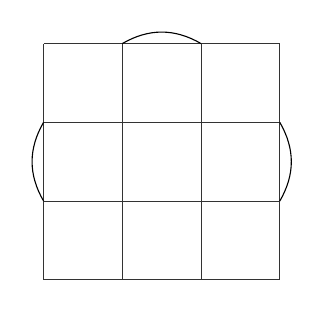
\begin{tikzpicture}
			\draw[step=1,black!80] (0,0) grid (3,3);
			\draw (0,1) to[bend left](0,2);	
			\draw (1,3) to[bend left](2,3);	
			\draw (3,2) to[bend left](3,1);	
		\end{tikzpicture}
		\caption{$13.5$ км в \ref{katok}}
	\end{minipage}
	\begin{minipage}{0.32\textwidth}\centering
		\setchessboard{showmover=false,setpieces={Qa1,Qd2,Qb3,Qe4,Qc5}}
		\chessboard[maxfield=e5]
		\caption{5 ферзей на доске $5\times5$}
	\end{minipage}
	\begin{minipage}{0.38\textwidth}\centering
		\setchessboard{showmover=false,setpieces={Qa3,Qb6,Qc2,Qd7,Qe5,Qf1,Qg8,Qh4}}
		\chessboard
		\caption{8 ферзей на доске $8\times8$}
	\end{minipage}
\end{figure}

\hrule\vskip10pt\hdr{Дорешка}

\z Двое играют на доске $10\times10$, за ход нужно положить на любые две соседние клетки доминошку так, чтобы доминошки не перекрывались. Проигрывает тот, кто не может сделать ход. Кто выиграет при правильной игре и как он должен играть, чтобы победить?

\s Второй выигрывает стратегией <<сделать ход, центрально-симметричный (относительно центра доски) последнему ходу первого>>. \QEDA\\

\n Дано $2019$ целых чисел. Известно, что сумма любых $100$ из них положительна. Верно ли, что сумма всех чисел положительна?

\s Это верно. Действительно, отрицательных чисел не больше $99$ (иначе можно взять $100$ отрицательных чисел и их сумма отрицательна). Поместим их в одну сотню. Сумма этой сотни положительна, а всех оставшихся чисел неотрицательна, значит, сумма всех чисел положительна. \QEDA

\p $2019$ целых чисел стоят в ряд. Известно, что сумма любых $100$ последовательно стоящих чисел положительна. Верно ли, что сумма всех чисел положительна?

\s Это неверно. Приведем пример, когда это не так. Разделим $2019$ на <<комплекты>> по $19$ чисел и $81$ числу. Пусть в каждом из <<комплектов>> числа равны, сумма чисел в каждом из комплектов из $19$ чисел будет равна $-a$, а в каждом комплекте из $81$ числа будет равна $a+1$ (например, подойдёт, если в <<малых>> комплектах все числа $-17$, а в <<больших>> $4$). Теперь поставим их в таком порядке: $19,81,\ldots,19$.Тогда в каждой сотне сумма равна $1$, и при нашем выборе чисел общая сумма $-303<0$. \QEDA\\

\newpage
\n Есть $n$ камешков, различных по весу, и двухчашечные весы без гирь. Как за наименьшее число взвешиваний найти самый тяжелый камешек, если на весы можно класть только по одному камню?\footnote{\textit{Примечание.} На самом деле, ответ не меняется, если можно класть больше одного камня за раз. Это можно доказать так. Пусть веса камней --- $10-1,10-\frac12,10-\frac14,\ldots,10-2^{n-1}$. Тогда если класть разное количество камней на весы, то они будут показывать, где больше камней, а если одинаковое --- перевешивать будет чаша, где нет минимального камня из лежащих на весах. Пусть вместо взвешивания к нам будет подходить шпион и, если количество камней одинаково, будет показывать на минимальный камень, тогда мы получим заведомо не меньше информации. Тогда ясно, что меньше чем $n-1$ взвешиванием не обойтись.}

\s Нужно $n-1$ взвешивание. Возьмем любую пару камней, определим самый тяжелый из них. Самый тяжелый будем взвешивать с любым из невзвешенных камней. В полученной паре определяем самый тяжелый и снова взвешиваем с одним из невзвешенных. Повторяем это до тех пор, пока не взвесим все камни. Легко понять, что это оптимальный алгоритм. \QEDA

\p Есть $68$ камешков, различных по весу, и двухчашечные весы без гирь. Как за $100$ взвешиваний найти самый тяжёлый и самый лёгкий камни?

\s Разобьем все камни по парам и камни в каждой паре сравним между собой. На это мы потратим $34$ взвешивания. Самые тяжелые отложим в одну сторону, а самые легкие в другую. Теперь нам нужно $n-1$ взвешивание на каждую из кучек (по алгоритму из прошлого пункта), т.е. $33$ на каждую. На это мы потратим $34+66=100$ взвешиваний. \QEDA\\

\z Петя заметил, что у всех его 25 одноклассников различное число друзей в этом классе. Сколько друзей в классе у Пети? (Найдите все решения).

\s Рассмотрим Васю --- одноклассника Пети, у которого больше всего друзей, и Колю --- одноклассника, у которого меньше всего друзей. Заметим, что либо у Коли 0 друзей, либо у Васи все ученики класса (кроме него самого) --- друзья. В обоих случаях Вася дружит с Петей, а Коля нет. Уберём из класса Васю и Колю. Все количества друзей у одноклассников Пети снова различны, у Пети теперь на 1 друга меньше, в классе на 2 человека меньше. Так можно сделать 12 раз, после чего останется Петя и ещё один человек. Они либо дружат, либо нет, причём оба варианта возможны. Ответ: 12 или 13.\QEDA\\

\z Двое играют в такую игру: имеется куча из 21 камня, ходят по очереди, за ход игрок забирает из кучи 1, 2 или 4 камня. Выигрывает тот, кто возьмёт последний камень. Кто выиграет при правильной игре и как ему играть?

\s Докажем, что первый проигрывает тогда и только тогда, когда текущее количество камней делится на 3. Действительно, если оно не делится, то можно вычесть 1 или 2 так, чтобы оно разделилось, а если делится, то в любом случае после хода делиться не будет. Кроме того, если камней 0, то проигрывает первый. Сейчас камней 21, это число делится на 3, значит, выигрывает второй.\QEDA

\end{document}
